\documentclass{article}
\usepackage[left=35mm,top=26mm,right=26mm,bottom=15mm]{geometry}
\usepackage[utf8]{inputenc}
\usepackage{graphicx}
\usepackage[normalem]{ulem}
\usepackage{amsmath}
\usepackage{verbatim}
\usepackage{mathrsfs}

%\usepackage{centernot}
\newcommand{\volume}{\mathop{\ooalign{\hfil$V$\hfil\cr\kern0.08em--\hfil\cr}}\nolimits}
\def\doubleunderline#1{\underline{\underline{#1}}}

\title{\textbf{\Huge AE 225}}
\author{\textbf{\Huge KRISHNA WADHWANI- 160010031} }
\date{\textbf{\huge \textit{NOVEMBER 1, 2017}}}

\begin{document}

\maketitle
\bigbreak
\bigbreak
\bigbreak

\section{\Large QUESTION 1}

Assumptions: 
\begin{itemize}
    \item Liquid is incompressible
    \item Flow of liquid jet is 1-D at inlet
    \item No fluid motion within the control volume relative to it
\end{itemize}

\noindent \underline{Step 1: Choosing Control Volume}\\

\noindent I am taking the tank as my control-volume (highlighted in red in the figure below). The selected control volume is moving with an accelerated velocity. At a give time t, it's velocity is $\underline{U}$. Mass of the system at any time t is $M$. Liquid jet is entering the tank with velocity $V \ \hat{\underline{i}}$ .\\
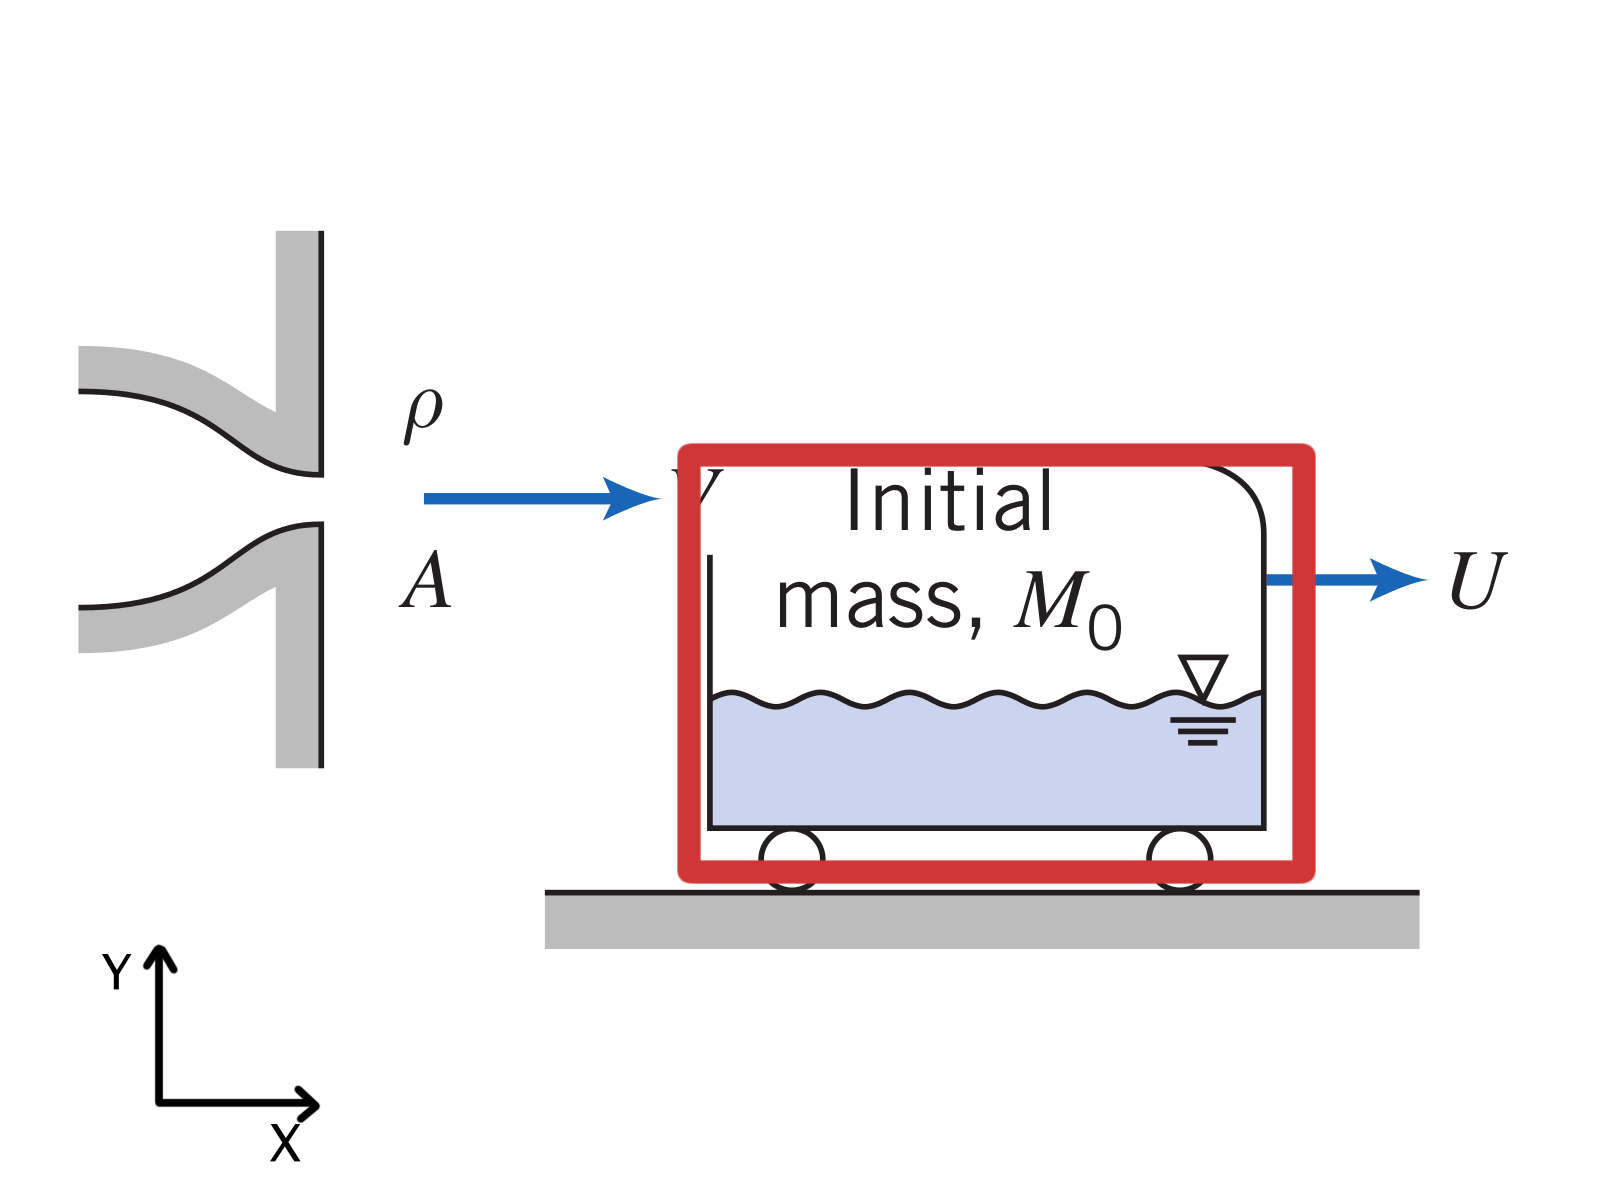
\includegraphics[scale=0.6]{225q12.png}

\noindent \underline{Step 2: Mass Conservation}\\

\noindent From Reynold Transport Theorem for mass consevation:\ 
$\frac{dm_{sys}}{dt}= \frac{\partial}{\partial t} \int\limits_{CV} \rho d\volume + \int\limits_{CS} \rho (\underline{W}.\hat{n})dA $

As mass of the system is conserved: $\frac{dm_{sys}}{dt}=0$ \\ 
$\implies \dfrac{dM}{dt} + \int\limits_{in} \rho (\underline{W}.\hat{n})dA + \int\limits_{out} \rho (\underline{W}.\hat{n})dA=0 $\\

$\int\limits_{out}\rho (\underline{W}.\hat{n})dA=0$ as air is deflected into the tank and not exiting it\\ 

$\int\limits_{in}\rho (\underline{W}.\hat{n})dA= -\rho A(V- U)$ as flow is 1-D\\
So, $\dfrac{dM}{dt}- \rho A(V- U)=0 \ \ \  \hdots eq^n 1$ \\
\newpage
\noindent \underline{Step 3: Momentum Conservation}\\

\noindent From Reynold Transport Theorem for momentum consevation:\ 
$\underline{F}= \frac{\partial}{\partial t} \int\limits_{CV} \rho\underline{V} d\volume + \int\limits_{CS} \rho (\underline{W}.\hat{n})\underline{V}dA $

Given negligible resistance, there is no net force on the control volume. So, what we get is(Assuming negligible flow of liquid inside the tank relative to the tank): \\
$\dfrac{d(MU)}{dt}+ \int\limits_{in} \rho (\underline{W}.\hat{n})\underline{V}dA=0$\\
$\implies M\dfrac{dU}{dt}+ U\dfrac{dM}{dt}- \rho(V-U)VA=0 $\\
Using  $eq^n 1$, we get:\\

$\dfrac{dU}{dt}= \dfrac{\rho A(V-U)^2}{M}  \ \ \ \hdots eq^n 2$ \\

Now using $eq^n 2$ for solving $eq^n 1$:\\

$dM= \rho A (V-U) \dfrac{dU}{dU/dt} $\\
$\implies \int\limits_{M_0}^M\dfrac{dM}{M}= \int\limits_0^{U}\dfrac{dU}{V-U} $\\
$\implies ln\dfrac{M}{M_0}=- ln\dfrac{\rvert V-U \rvert}{V}$\\
\bigbreak
\noindent $\implies \mathbf{M=\dfrac{M_0} {V-U} }$\\
\bigbreak
\noindent Using the value of M, we get:\\
$\dfrac{dU}{dt}= \dfrac{\rho A(V-U)^3}{M_0V}$\\
$\implies \int\limits_0^U\dfrac{dU}{(V-U)^3}=\int\limits_0^t \dfrac{\rho Adt}{M_0V}$\\
$\implies \dfrac{1}{2}\Big[\dfrac{1}{(V-U)^2}- \dfrac{1}{V^2}\Big]=\dfrac{\rho At}{M_0V}$\\
$\implies \dfrac{1}{\bigg(1-\dfrac{U}{V} \bigg)^2}= \dfrac{2\rho AVt}{M_0}+ \dfrac{1}{v^2}$\\
\bigbreak
$\mathbf{\implies \dfrac{U}{V}= 1-\dfrac{1}{\bigg( 1+ \dfrac{2\rho AVt}{M_0}\bigg)^{1/2}}}$


\newpage
\section{\Large QUESTION 2}

Assumptions: 
\begin{itemize}
    \item Air is \underline{incompressible} at standard condition
    \item Flow is \underline{steady}
    \item Flow is \underline{1-D}
\end{itemize}
\bigbreak

\noindent To calculate pressure at inlet, I am using Bernoulli's equation at a point on the atmosphere and a point on inlet at the same streamline:\\
$\dfrac{P}{\rho}+\dfrac{v^2}{2}+gz=c$\\
Assuming velocity of the air at atmosphere to be zero and taking the two points at same height:\\
$P_{atm}=P_1+\dfrac{\rho V_1^2}{2}$\\
$\implies P_{in,gauge}=-\dfrac{\rho V_1^2}{2}$\\


\noindent \underline{Step 1: Choosing control volume}\\

\noindent The chosen control volume is as follows (highlighted in red in the figure below). Chosen control volume is perpendicular to the flow. Air is entering the control volume with a velocity $-V_{in} \ \hat{\underline{j}}$ and exiting the control volume with velocity $-V_{out} \ \hat{\underline{j}}$ \\
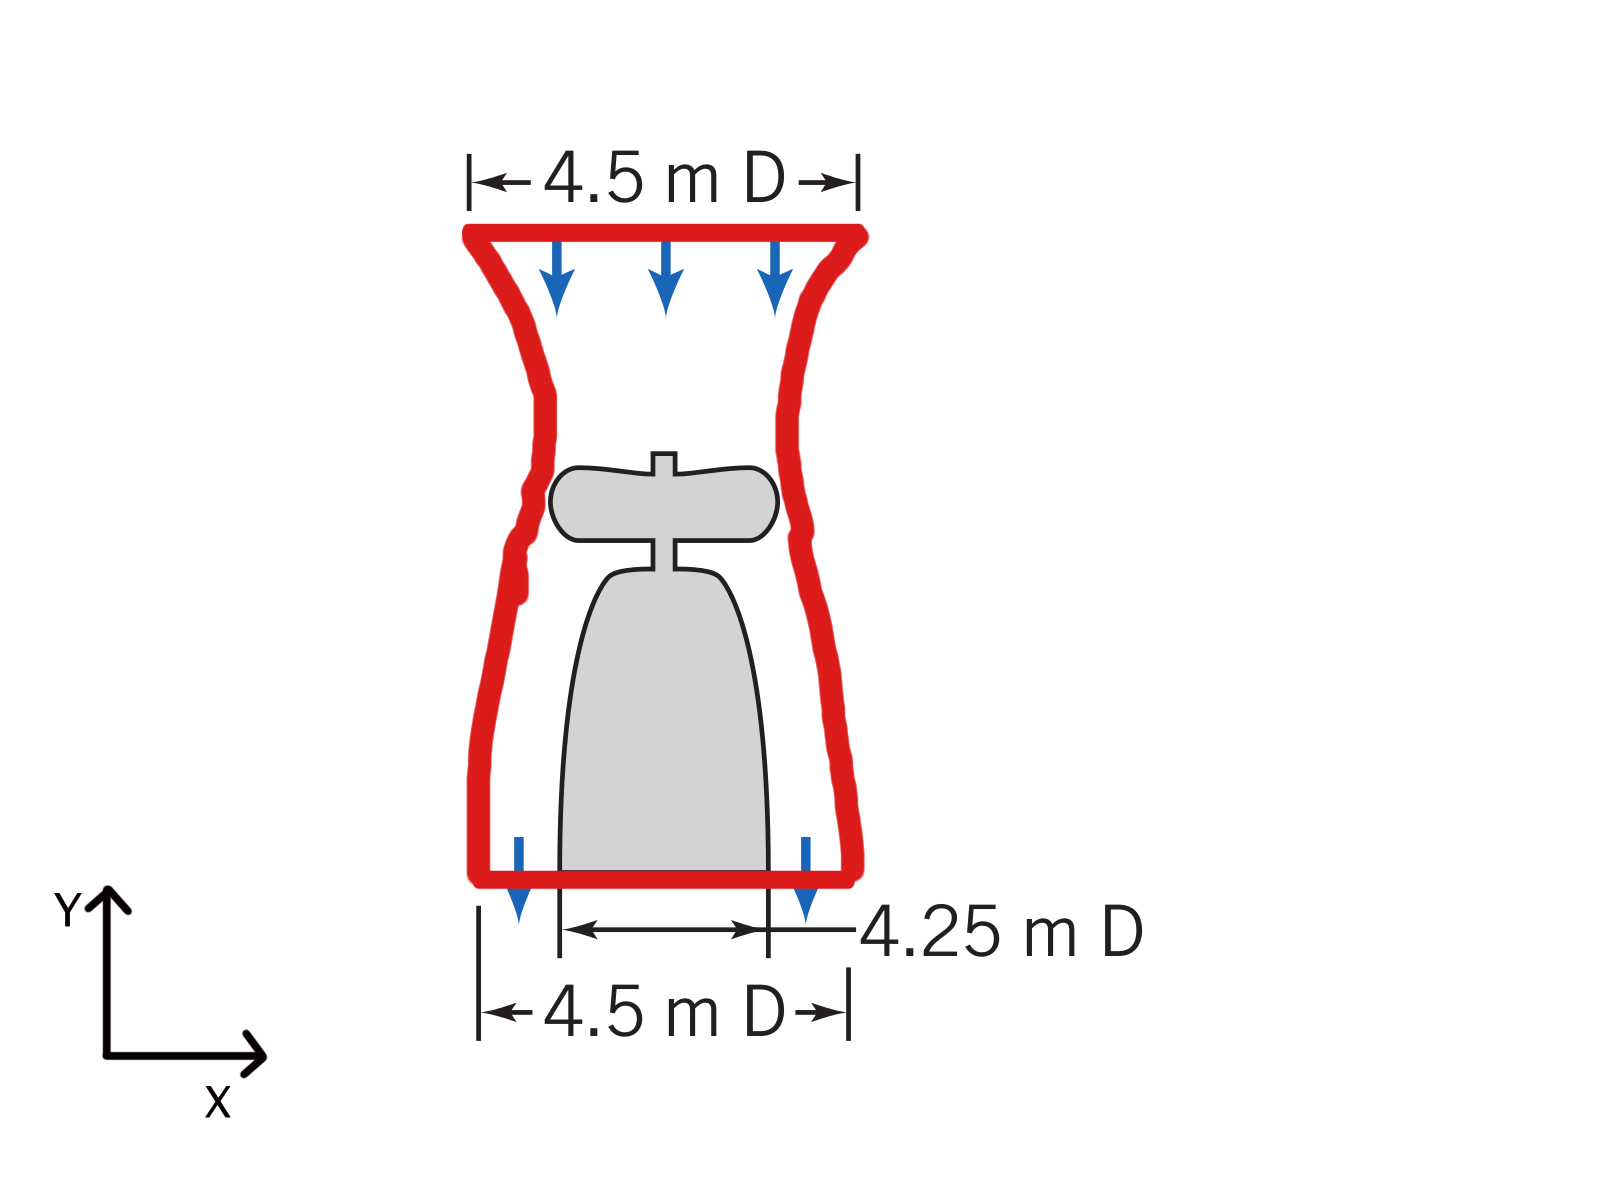
\includegraphics[scale=0.6]{225q2.png}

\noindent \underline{Step 2: Mass Conservation}\\

\noindent From Reynold Transport Theorem for mass consevation:\ 
$\frac{dm_{sys}}{dt}= \frac{\partial}{\partial t} \int\limits_{CV} \rho d\volume + \int\limits_{CS} \rho (\underline{W}.\hat{n})dA $

\noindent As mass of the system is conserved: $\frac{dm_{sys}}{dt}=0$ \\ 
As flow is steady: $\dfrac{\partial}{\partial t} \int\limits_{CV} \rho d\volume =0$\\
As flow is 1D and incompressible: $\int\limits_{CS} \rho (\underline{W}.\hat{n})dA= \rho A_{out}V_{out} - \rho A_{in}V_{in}$\\
$\implies A_{out}V_{out}= A_{in}V_{in} \ \ \ \hdots eq^n 1$\\

\noindent \underline{Step 3: Momentum Conservation}\\

\noindent Momentum consevation along $y$:\\ 
$\underline{F}= \frac{\partial}{\partial t} \int\limits_{CV} \rho\underline{V} d\volume + \int\limits_{CS} \rho (\underline{W}.\hat{n})\underline{V}dA $\\

\noindent As flow is steady: $\frac{\partial}{\partial t} \int\limits_{CV} \rho\underline{V} d\volume=0$\\
As flow is 1-D and incompressible: $\int\limits_{CS} \rho (\underline{W}.\hat{n})\underline{V}dA= \rho A_{in} V_{in}^2- \rho A_{out}V_{out}^2$

\noindent Net force on the control volume is equal to the weight of the helicopter = $-mg-P_{in,gauge}A_{in}+P_{out,gauge}A_{out}$\\
$\implies -mg-(-\dfrac{\rho V^2}{2})A_{in}+0= \rho A_{in} V_{in}^2- \rho A_{out}V_{out}^2 $\\
From $eq^n 1$: \\
$\implies -mg+\dfrac{\rho V_{in}^2}{2}A_{in}= \rho A_{in}V_{in}^2(1-\dfrac{A_{in}}{A_{out}})$\\
$\implies V_{in}^2= -\dfrac{mg}{-\dfrac{\rho A_{in}}{2} + \rho A_{in}(1-\dfrac{A_{in}}{A_{out}})}$\\

\noindent Given: \\
${A_{in}=\dfrac{\pi (4.5)^2}{4}} = 15.904 m^2$ \\
$A_{out}= \dfrac{\pi[(4.5)^2- (4.25)^2]}{4} = 1.718 m^2 $\\
$m=1000kg$\\
Taking: 
$g=9.81m/s^2$, \
$\rho = 1.225 kg/m^3$

\noindent Using these values in the above expression, we get: $V_{in}= 7.58 \ m/s^2$\\
\noindent So, we get speed of the air leaving the craft $V_{out}$ as: \\

$V_{out}= \dfrac{A_{in}V_{in}}{A_{out}}$\\
$\mathbf{\implies V_{out}= 70.2\  m/s^2}$\\

\noindent \underline{Step 4: Energy Conservation} \\
For the minimum power(denoted by $\dot{\mathscr{W}}_{shaft,net,in}$) delivered by the propeller, we will use energy conservation equation as: 

$\dfrac{d}{dt}\int\limits_{CV}e\rho\volume + \int\limits_{CS} ( \check{u} + \dfrac{p}{\rho}+ \dfrac{V^2}{2}+ gz)\rho(W.\hat{n})dA = \dot{\mathscr{W}}_{shaft,net,in} +\dot{\mathscr{Q}}_{net,in}$\\

\noindent Applying assumptions of 1D inlet/outlet, steady, incompressibility and no heat input, we get: \\
$ \rho A_{in}V_{in}(\check{u}_{out}- \check{u}_{in} +  \dfrac{V_{out}^2- V_{in}^2}{2} + g\Delta z +\dfrac{P_{out}-P_{in} }{\rho}) =\dot{\mathscr{W}}_{shaft,net,in}$\\

\noindent Using equation of state:$P=\rho RT$: $T_1=288.1K$ and $T_2=288.0026K$. As change in temperature is small, we can neglect changes in internal energy as internal energy is a function of temperature. $P_{out}-P_{in}=\dfrac{\rho V_1^2}{2}$\\ Ignoring changes in gravitational potential energy: \\ 

\noindent $\implies \dot{\mathscr{W}}_{shaft,net,in}= \rho A_{out}\dfrac{V_{out}^3}{2} $\\
Placing the values, We get:\\
$\mathbf{\dot{\mathscr{W}}_{shaft,net,in}= 363.89 \ kW} $

\newpage
\section{\Large QUESTION 3}

Incompressible Navier-Stoke's equations: \\

\noindent Mass conservation: $\nabla.\underline{u}=0$\\
Momentum Conservation: $\rho \dfrac{\partial u}{\partial t} + \rho (\underline{u}. \nabla) \underline{u})= -\nabla p +\underline{f}_{body} +\mu \nabla^2 \underline{u} $\\
\bigbreak 
\noindent In cylindrical coordinates: \\
 
\noindent Mass conservation: $\dfrac{1}{r} \dfrac{\partial (ru_r)}{\partial r} + \dfrac{1}{r} \dfrac{\partial u_\theta}{\partial \theta}+ \dfrac{\partial u_z}{\partial z}=0$\\
Momentum conservation: \\
Along $r$: $\rho (\dfrac{\partial u_r}{\partial t}+ u_r\dfrac{\partial u_r}{\partial r} + \dfrac{u_\theta}{r}\dfrac{\partial u_r}{\partial \theta} - \dfrac{u_\theta^2}{r}+ u_z\dfrac{\partial u_r}{\partial z}) = -\dfrac{\partial P}{\partial r}+ \rho g_r + \mu[\dfrac{1}{r}\dfrac{\partial}{\partial r}(r\dfrac{\partial u_r}{\partial r}) - \dfrac{u_r}{r^2} + \dfrac{1}{r^2}\dfrac{\partial^2 u_r}{\partial \theta^2} - \dfrac{2}{r^2}\dfrac{\partial u_\theta}{\partial \theta}+ \dfrac{\partial^2 u_r}{\partial z^2}]$\\

\noindent Along $\theta$: $\rho (\dfrac{\partial u_\theta}{\partial t}+ u_r\dfrac{\partial u_\theta}{\partial r} + \dfrac{u_\theta}{r}\dfrac{\partial u_\theta}{\partial \theta} + \dfrac{u_\theta u_r}{r}+ u_z\dfrac{\partial u_\theta}{\partial z}) = -\dfrac{1}{r}\dfrac{\partial P}{\partial \theta}+ \rho g_\theta + \mu[\dfrac{1}{r}\dfrac{\partial}{\partial r}(r\dfrac{\partial u_\theta}{\partial r}) - \dfrac{u_\theta}{r^2} + \dfrac{1}{r^2}\dfrac{\partial^2 u_\theta}{\partial \theta^2} + \dfrac{2}{r^2}\dfrac{\partial u_r}{\partial \theta}+ \dfrac{\partial^2 u_\theta}{\partial z^2}]$\\

\noindent Along $z$: $\rho (\dfrac{\partial u_z}{\partial t}+ u_r\dfrac{\partial u_z}{\partial r} + \dfrac{u_\theta}{r}\dfrac{\partial u_z}{\partial \theta} + u_z\dfrac{\partial u_z}{\partial z}) = -\dfrac{\partial P}{\partial z}+ \rho g_z + \mu[\dfrac{1}{r}\dfrac{\partial}{\partial r}(r\dfrac{\partial u_z}{\partial r}) + \dfrac{1}{r^2}\dfrac{\partial^2 u_z}{\partial \theta^2} + \dfrac{\partial^2 u_z}{\partial z^2}]$\\

\noindent Assumptions to obtain exact solution for cylinderical coulette flow: 
\begin{itemize}
    \item Laminar
    \item Incompressible
    \item Steady
    \item Rotationally Symmetric ($\approx$\ Fully developed)
    \item Simple Geometry
    \item Ignoring gravity
\end{itemize}

\noindent From the above conditions: \\

$\dfrac{\partial P}{\partial \theta}=0, \dfrac{\partial P}{\partial z}=0$\\

\noindent Although rotationally assymetric solution also exists, we concern our self with rotationally symmetric solution for our problem. As flow is rotationally symmetric and there is no flow in axial direction, velocity will depend only on $r$ and $u_z=0$. So, our velocity is of the form: 

$\underline{u}=u_r(r)\hat{e}_r + u_\theta(r)\hat{e}_\theta$\\

\noindent \underline{Applying mass conservation}: \\ 
$\nabla.(\underline{u})=0$\\
$\implies \dfrac{1}{r} \dfrac{\partial (ru_r)}{\partial r} + \dfrac{1}{r} \dfrac{\partial u_\theta}{\partial \theta}+ \dfrac{\partial u_z}{\partial z}=0$ \\
Now, \\
$\dfrac{\partial u_\theta}{\partial \theta}=0$\ as $u_\theta$ is a function of $r$ due to rotational symmetry \\
$\dfrac{\partial u_z}{\partial z}=0$\ as $u_z$ due to no flow in axial direction\\
$\implies \dfrac{1}{r} \dfrac{d(ru_r)}{dr}=0$\\
Integrating with respect to $r$:\\
$ru_r=k$\\
As $u_r=0$ at $r=R_1$ and $r=R_2$,\\ $u_r \equiv 0$

\noindent \underline{Momentum conservation along $r$:}\\
$\rho (\dfrac{\partial u_r}{\partial t}+ u_r\dfrac{\partial u_r}{\partial r} + \dfrac{u_\theta}{r}\dfrac{\partial u_r}{\partial \theta} - \dfrac{u_\theta^2}{r}+ u_z\dfrac{\partial u_r}{\partial z}) = -\dfrac{\partial P}{\partial r}+ \rho g_r + \mu[\dfrac{1}{r}\dfrac{\partial}{\partial r}(r\dfrac{\partial u_r}{\partial r}) - \dfrac{u_r}{r^2} + \dfrac{1}{r^2}\dfrac{\partial^2 u_r}{\partial \theta^2} - \dfrac{2}{r^2}\dfrac{\partial u_\theta}{\partial \theta}+ \dfrac{\partial^2 u_r}{\partial z^2}]$\\

\noindent $\rho \dfrac{\partial u_r}{\partial t}=0$\ as flow is steady\\$u_r\dfrac{\partial u_r}{\partial r}=0$\ as $u_r=0$\\
$\dfrac{u_\theta}{r}\dfrac{\partial u_r}{\partial \theta}=0$ as $u_r=u_r(r)=0$\\
$u_z\dfrac{\partial u_r}{\partial z}=0$\ as $u_r=u_r(r)=0$\\
$\rho g_r=0\  $ as $g $\ is along $z$ \\
$\dfrac{1}{r}\dfrac{\partial}{\partial r}(r\dfrac{\partial u_r}{\partial r})$\ as $u_r=0$\\
$\dfrac{u_r}{r^2}=0$\ as $u_r=0$\\
$\dfrac{\partial^2 u_r}{\partial \theta^2}=0$ as $u_r=u_r(r)=0$\\
$\dfrac{\partial u_\theta}{\partial \theta}=0$\ as $u_\theta=u_\theta(r)$ \\
$\dfrac{\partial^2 u_r}{\partial z^2}=0$\ as there is no flow in radial direction\\

\noindent So, we get: \\

\noindent $\rho \dfrac{u_\theta}{r^2}= -\dfrac{\partial P}{\partial r}$\\

\noindent \underline{Momentum conservation along $z$:}\\
$\rho (\dfrac{\partial u_z}{\partial t}+ u_r\dfrac{\partial u_z}{\partial r} + \dfrac{u_\theta}{r}\dfrac{\partial u_z}{\partial \theta} + u_z\dfrac{\partial u_z}{\partial z}) = -\dfrac{\partial P}{\partial z}+ \rho g_z + \mu[\dfrac{1}{r}\dfrac{\partial}{\partial r}(r\dfrac{\partial u_z}{\partial r}) + \dfrac{1}{r^2}\dfrac{\partial^2 u_z}{\partial \theta^2} + \dfrac{\partial^2 u_z}{\partial z^2}]$\\

\noindent $\rho \dfrac{\partial u_z}{\partial t}=0$\ as flow is steady \\
\noindent $u_r\dfrac{\partial u_z}{\partial r}=\dfrac{u_\theta}{r}\dfrac{\partial u_z}{\partial \theta}=u_z\dfrac{\partial u_z}{\partial z}) = \dfrac{1}{r}\dfrac{\partial}{\partial r}(r\dfrac{\partial u_z}{\partial r})= \dfrac{1}{r^2}\dfrac{\partial^2 u_z}{\partial \theta^2}=\dfrac{\partial^2 u_z}{\partial z^2}=0$ as $u_z=0$ (No flow in $z$ direction) \\
$\dfrac{\partial P}{\partial z} =0$ \ as give that there is no flow in axial direction \\
$\rho g_z=0$ as we have ignored gravity \\

\noindent \underline{Momentum conservation along $\theta$:}\\

\noindent $\rho (\dfrac{\partial u_\theta}{\partial t}+ u_r\dfrac{\partial u_\theta}{\partial r} + \dfrac{u_\theta}{r}\dfrac{\partial u_\theta}{\partial \theta} + \dfrac{u_\theta u_r}{r}+ u_z\dfrac{\partial u_\theta}{\partial z}) = -\dfrac{1}{r}\dfrac{\partial P}{\partial \theta}+ \rho g_\theta + \mu[\dfrac{1}{r}\dfrac{\partial}{\partial r}(r\dfrac{\partial u_\theta}{\partial r}) - \dfrac{u_\theta}{r^2} + \dfrac{1}{r^2}\dfrac{\partial^2 u_\theta}{\partial \theta^2} + \dfrac{2}{r^2}\dfrac{\partial u_r}{\partial \theta}+ \dfrac{\partial^2 u_\theta}{\partial z^2}]$\\

\noindent $\rho \dfrac{\partial u_{\theta}}{\partial t}=0$\ as flow is steady \\
$u_r\dfrac{\partial u_\theta}{\partial r}=\dfrac{u_\theta u_r}{r}=\dfrac{2}{r^2}\dfrac{\partial u_r}{\partial \theta}=0$ as $u_r=u_r(r)=0$\\
$\dfrac{u_\theta}{r}\dfrac{\partial u_\theta}{\partial \theta}=u_z\dfrac{\partial u_\theta}{\partial z}) = \dfrac{1}{r^2}\dfrac{\partial^2 u_\theta}{\partial \theta^2}=\dfrac{\partial^2 u_\theta}{\partial z^2}=0$ as $u_{\theta}= u_{\theta}(r)$\\
$\rho g_{\theta}=0\  $ as $g $\ is along $z$\\

\noindent So, we get :\\
$\dfrac{\partial}{\partial r}\Big (\dfrac{1}{r}\big (\dfrac{\partial (ru_\theta)}{\partial r}\big )\Big )=0$\\
As $u_\theta$ is a function of $r$:\\
$\dfrac{d}{d r}\Big (\dfrac{1}{r}\big (\dfrac{d (ru_\theta)}{d r}\big )\Big )=0$\\
Integrating with respect to $r$:\\
$\dfrac{1}{r}\dfrac{d(ru_\theta)}{dr}=c_1$\\
$\implies u_\theta(r)= \dfrac{c_1r}{2}+ \dfrac{c_2}{r}$
\bigbreak

\noindent Applying boundary conditions(No-slip condition): \\
$u_\theta=\omega_1 R_1$ \ for $r=R_1$\\
$u_\theta=\omega_2 R_2$ \ for $r=R_2$\\
From these 2 conditions, we get: \\
$c_1=2\dfrac{\omega_1 R_1^2- \omega_2R_2^2}{R_1^2-R_2^2}$\\
$c_2=-R_1^2R_2^2\dfrac{\omega_1-\omega_2}{R_1^2-R_2^2}$\\
With these values, we obtain the velocity field of the cylinder as: \\
$\mathbf{\underline{u}= \dfrac{\omega_2R_2^2- \omega_1R_1^2}{R_2^2-R_1^2}r\ + \dfrac{1}{r}\dfrac{R_1^2R_2^2(\omega_1-\omega_2)}{R_2^2-R_1^2} \ \hat{e}_\theta}$
\bigbreak

\noindent \underline{Evaluating wall sheer stress at the two walls}\\
$\tau= 2\mu \doubleunderline{\epsilon}$\\
Where $\doubleunderline{\epsilon}= \dfrac{1}{2}(\nabla u + (\nabla u) ^T)$\\
In a general coordinate system($x_1,x_2,x_3$), we have: \\
$\tau_{ij}=\mu(\dfrac{\partial u_i}{\partial x_j} + \dfrac{\partial u_j}{\partial x_i})$

\noindent However, for the give problem: $u_r=0, u_z=0$ and $u_\theta=u_\theta(r)$. So, only one term of the tensor $\tau_{r\theta}$ remains. For cylindrical coordinates, we get- \\
$\tau_{r\theta}=\mu\Big (\dfrac{du_\theta}{dr}- \dfrac{u_{\theta}}{r} +\dfrac{1}{r}\dfrac{\partial u_r}{\partial \theta} \Big )$\\
As $u_r=u_r(r)=0$:\\

\noindent$\implies \tau_{r\theta}=\mu\Big (\dfrac{\omega_2 R_2^2- \omega_1R_1^2}{R_2^2-R_1^2} -\dfrac{1}{r^2}\dfrac{R_1^2R_2^2(\omega_1-\omega_2)}{R_2^2-R_1^2} - \dfrac{\omega_2R_2^2- \omega_1R_1^2}{R_2^2-R_1^2}\ - \dfrac{1}{r^2}\dfrac{R_1^2R_2^2(\omega_1-\omega_2)}{R_2^2-R_1^2} \  \Big ) $ \\
$\implies \tau_{r\theta}=\mu\Big (-\dfrac{2}{r^2}\dfrac{R_1^2R_2^2(\omega_1-\omega_2)}{R_2^2-R_1^2} \  \Big ) $ \\

\noindent At inner wall($r=R_1$):\\
$\mathbf{\tau_{w}\bigg\rvert_{r=R_1}= \dfrac{2\mu R_2^2(\omega_2-\omega_1)}{R_2^2-R_1^2}}$\\

\noindent At outer wall($r=R_2$):\\
$\mathbf{\tau_{w}\bigg\rvert_{r=R_2}= \dfrac{2\mu R_1^2(\omega_2-\omega_1)}{R_2^2-R_1^2}}$\\

\bigbreak
\bigbreak

\end{document}
